\chapter{Wrapped Illustrations}
\label{ch:wrapped}
\parindent2em
\let\onepar\lorem

Wrapped figures are not in vogue and most users of \latex avoid them.
If you are planning to have a more traditional book design wrapped figures might be more appropriate. Traditional typographers used
all sorts of styles to achieve wrapped figures which conserved paper. 
The best way to achieve it is to use Donald Arseneau's |wrafig| package \citep{wrapfig}.

\begin{wrapfigure}{l}{3.2cm}
    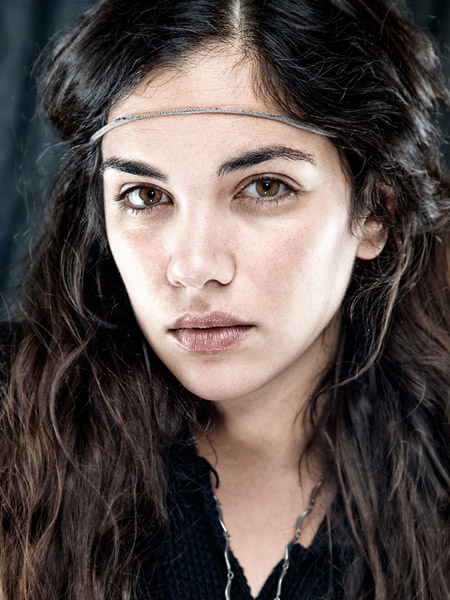
\includegraphics[width=3cm]{./images/amato.jpg}
    \caption{\footnotesize Wrapped figures}
\end{wrapfigure}

Get prepared to do a lot of manual adjustments, see your figures disappear on page refreshes and reruns. It is also recommended that you do your final adjustments once you are happy with the contents of your document and these final adjustments will not start jumping around. 
After a while though you get the hang of it and by minor adjustments you can really achieve great results. The manual uses \verb+everypar+ to insert commands for the shaping of the paragraphs that \emph{follow} the wrapped figure.

The package provides the environments \pkg{wrapfigure} and \pkg{wraptable} for typesetting a
narrow float at the edge of the text, and making the text wrap around it. The |wrapfigure|
and |wraptable| environments interact properly with the \verb+\caption+ command to produce
proper numbering, but they are not regular floats like \textit{figure} and \textit{table}, so be aware to do manual adjustments. If you do not take care 
they may also be printed out of sequence with the regular floats.

The |wrapfigure| environment  provides one of those monster locomotive type commands that stresses one's memory as it provides for four parameters.
 
The four param
for \verb+\begin{wrapfigure}+, two optional and two required, plus the text of the figure, with a caption perhaps.

\begin{macro}{wrapfigure}
\end{macro}

|\begin{wrapfigure}[12]{r}[34pt]{5cm}\meta{figure}\end{wrapfigure}|

  \begin{tikzpicture}[xshift=-15pt]
    \node (number) at (0mm, 0mm) {\oarg{number of narrow lines}};
    \node (placement) at (36mm, 0mm) {\marg{placement}};
    \node (overhang) at (60mm, 0mm) {\oarg{overhang}};
    \node (width) at (81mm, 0mm) {\marg{width}};
    \begin{scope}[->]
    \draw (number) -- (16mm, 17mm);
    \draw (placement) -- (24mm, 17mm);
    \draw (overhang) -- (35mm, 17mm);
    \draw (width) -- (47mm, 17mm);
    \end{scope}
  \end{tikzpicture}


First we will look at placing the figure without the use of optional commands.


\begin{verbatim}
\begin{wrapfigure}{r}{.4\textwidth}
    \includegraphics[width=.4\textwidth]{./path/file}
    \caption{\footnotesize Wrapped figures}
\end{wrapfigure}
\end{verbatim}

From the four parameters the first one indicates if the figure is to be typeset left or right.

\begin{verbatim}
\begin{wrapfigure}{l}{\imagewidth}
    \includegraphics[width=\imagewidth



]{./graphics/parasol-01}
    \caption{\footnotesize Wrapped figures}
\end{wrapfigure}
\end{verbatim}


\begin{wrapfigure}[18]{I}[0.1pt]{85pt}
    \captionsetup{name=Fig.}
    \vskip-10.5pt plus 2pt minus 2pt\relax
    \includegraphics[width=83pt]{./images/parasol-01.jpg}
    \caption{Wrapped figures, parameters set at \texttt\{l\}\{90pt\}.}
\end{wrapfigure}

Changing the parameters to suit we now have the illustration floating to the left. Allowing for the figure to be approximately two point  wider than the actual graphic, will leave a bit more margin. If the figure is end low in the page you need to be careful, that it does not disappear, as you will not get any warning.

The first parameter we are going to use an optional parameter is the one that determines the number of narrow lines. The format is \verb+[narrowlines]{l}{90pt}+. Think of this parameter as a fine tuning parameter and do not touch it until after your final draft is ready. If you see indented lines at the beginning of the page that follows the wrapped figure, reduce the number of lines, until you get satisfactory results.

The second optional parameter, comes after the \texttt{\{r\}[overhang]} parameter.

The second optional parameter (\#3) tells how much the figure should hang out into
the margin. The default overhang is given by the length \verb+\wrapoverhang+, which is 0pt
normally but can be changed using the command |\setlength|. For example, to have all wrapped figures you can 
use the space reserved for marginal notes,

\begin{verbatim}
\setlength{\wrapoverhang}{\marginparwidth}
\addtolength{\wrapoverhang}{\marginparsep}
\end{verbatim}

Again not recommended. The best approach is to specify the figures with \textbf{O} or \textbf{I}, let them float and if the results are
not very good then make manual adjustments. Get prepared to spend at least 5-10 minutes fiddling with the final result.

When you do specify the overhang explicitly for a particular figure, you can use a
special unit called \string\width meaning the width of the figure. For example, [0.5\string\width]
makes the center of the figure sit on the edge of the text, and [\string\width] puts the figure
entirely in the margin (and the adjacent text is indented by just \string\columnsep). This
\texttt{\string\width} is the actual width of the wrapfigure, which may be greater than the declared
width.

\begin{figure}[tb]
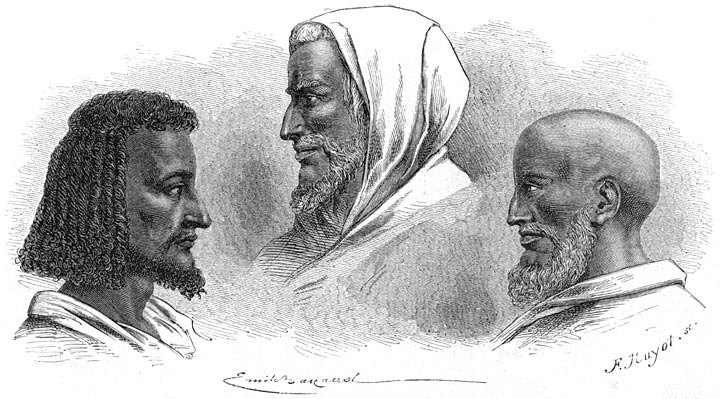
\includegraphics[width=\textwidth]{./graphics/chiefs.jpg}
\caption{Chiefs of Kelau or Kelaou.}
\label{fig:chiefs}
\end{figure}

\begin{figure}[p]
\centering

\includegraphics[width=0.8\textwidth,height=0.9\textheight, keepaspectratio]{./images/parasol-01.jpg}
\caption{Chiefs of Kelau or Kelaou.}
\label{fig:parasol-01}
\end{figure}

\section{Balancing the illustrations}

Illustrations come in various sizes, but in general they need to flow with the text. Place figures on top of the page and figures that would dominate the text on their own page. For example Figure~\ref{fig:chiefs} was allowed to float to the top of a page whereas Figure~\ref{fig:parasol-01} was placed on its own page, as I thought it will overwhelm the text if shown in a large size. However the same figure seems perfectly alright as a wrapped figure.

\begin{texexample}{}{}
\begin{wrapfigure}{I}{0pt}
    \includegraphics[width=75pt]{./images/parasol-01.jpg}
 \end{wrapfigure}
\lipsum[1-2]
\begin{wrapfigure}{l}{0pt}
    \includegraphics[width=75pt]{./images/parasol-01.jpg}
 \end{wrapfigure}
\lipsum[1-2]
\end{texexample}



\begin{texexample}{}{}
\begin{wrapfigure}{l}{0pt}
    \includegraphics[width=70pt]{./images/parasol-01.jpg}
    \includegraphics[width=70pt]{./images/parasol-01.jpg}
 \end{wrapfigure}

\lipsum[1-3]\lorem
\end{texexample}




\begin{texexample}{}{}
\begin{wrapfigure}[13]{L}{0pt}
    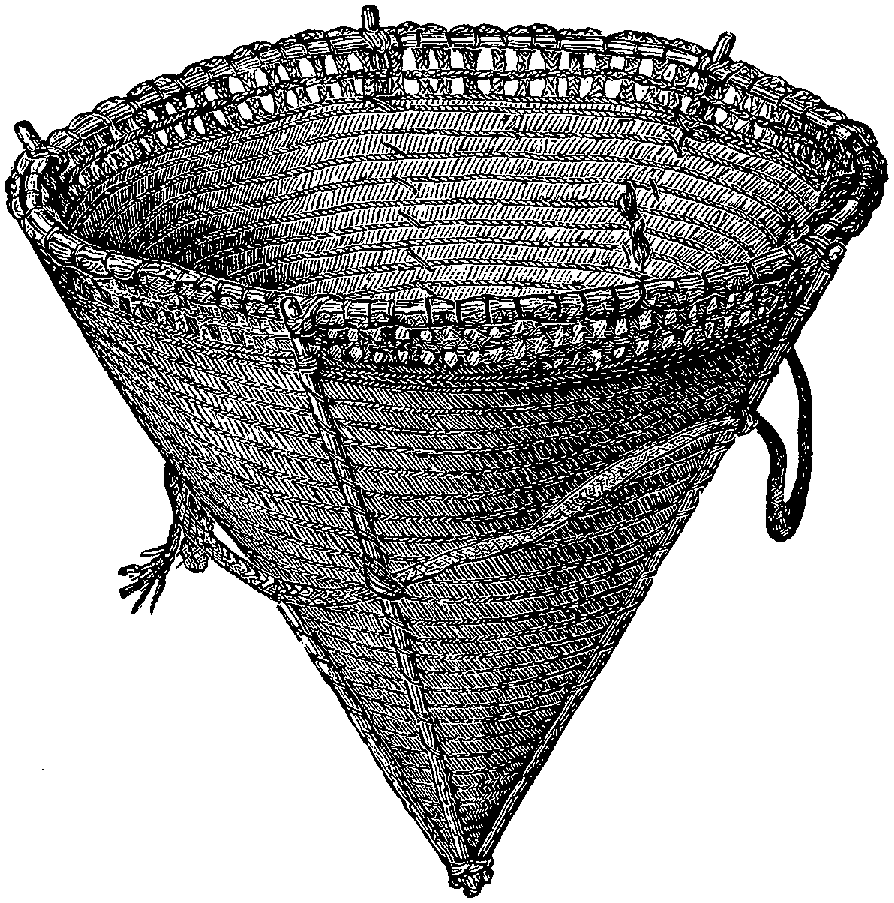
\includegraphics[width=100pt]{./graphics/conicalbasket.png}
\end{wrapfigure}

\onepar\onepar\onepar

\end{texexample}



